\chapter{Resultados de Integração}
Neste capítulo são apresentados os testes feitos com o intuito de alcançar
a integração entre os sistemas produzidos. Vale ressaltar que foram dispostos
de forma cronológica, facilitando a visão evolutiva do projeto.

\section{Integração}
A primeira  estrutura do robô, CPR-00, foi construída utilizando base de aço, cortada com uma esmerilhadeira nos moldes do design inicial e, em seguida, fixou-se as quatro rodas de locomoção laterais. Com a base pronta, realizou-se o primeiro teste, que foi a inserção da bomba na base para verificação da locomoção somente com propulsão da bomba d'água. Após a avaliação do primeiro teste, ficou evidenciado que a propulsão era eficiente, porém a utilização do material usado na base do robô sofreu corrosões devido ao contato do aço com o cloro da piscina. Com a finalidade de corrigir este problema, foi repensado a forma da base e o possível material a ser utilizado na nova fabricação da base do robô. Em paralelo, na parte de controle do robô foram realizados diversos testes na comunicação da \textit{raspberry pi} e Arduíno, bem como testes usando os componentes eletrônicos pela camada de serviço: servos motores do duto e rodas, acionamento da bomba e leitura de dados do sensor de pressão. O CPR-00 foi apresentado no segundo ponto de controle da disciplina.

\begin{figure}[h]
  \centering
  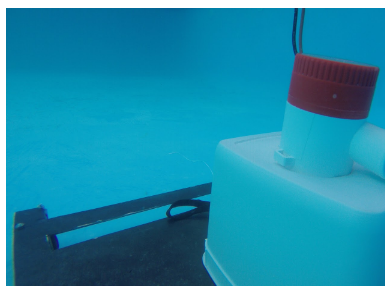
\includegraphics[width=0.6\textwidth]{figuras/test.png}
  \caption{Teste realizado no CPR-00}
  \label{fig:test}
\end{figure}
\FloatBarrier

O material comprado para confecção da estrutura da segunda versão do robô, CPR-01, consumiu 10 dias para entrega. Enquanto isso, a equipe confeccionou o duto de saída do jato, bem como as engrenagens para giro desse duto usando o servo. As escovas também foram ajustadas para a nova estrutura e, em paralelo, ocorreu os testes usando o sensor de distância, modelo HCSR04, isolado e imerso na água. Com esses testes, a equipe verificou que não seria possível utilizar esse modelo de sensor e, com isso, comprou-se e testou-se o modelo de sensor infravermelho E18-D0NK. Embora já houvesse uma implementação básica para percurso do robô cobrindo toda a área da piscina, utilizando máquina de estados, a camada de e a serviço implementada, foi realizada a implementação de um percurso simplificado de forma a auxiliar nos testes iniciais do protótipo. Nesse percurso simplificado, ocorre o acionamento da bomba d’água seguido da verificação constante do sensor de distância. Quando o sensor detecta algum obstáculo, a bomba é desligada e o servo motor do duto redireciona o jato d’água. Após esse momento, a bomba d’água é religada de forma a possibilitar a continuidade do movimento. A figura abaixo ilustra o percurso simplificado:

\begin{figure}[h]
  \centering
  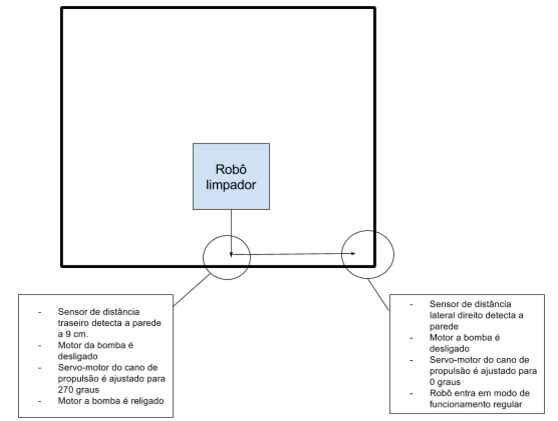
\includegraphics[width=0.8\textwidth]{figuras/cpr-01.png}
  \caption{Percurso para o teste}
  \label{fig:cpr-01}
\end{figure}
\FloatBarrier

Com a chegada do material comprado, iniciou a confecção da estrutura do CPR-01. Entretanto, o material era divergente do esperado, já que no lugar da placa de plástico adquirida foi entregue uma placa de poliestireno. Ainda assim, houve a construção de uma estrutura, conforme projetado. A principal dificuldade nessa construção foi a colagem desse material. Para isso, utilizou-se diversas alternativas como cola quente, superbonder, cola de isopor, adesivo ecológico, entre outras alternativas. No teste do CPR-01, essa estrutura foi invalidada por dois motivos: a colagem não se mostrou resistente para suportar os demais componentes e, ainda mais importante, o material é menos denso que a água, o que provoca a flutuação do robô.

Por fim, utilizou-se para a construção da nova carcaça uma adaptação de recipiente de plástico. Esta foi adaptada de acordo com o escopo definido, a fim de se realizar os testes do robô. O CPR-02 possui base e estrutura de plástico, rodas com liberdade de 360 graus, duto controlado pelo servo motor e dois filtros internos. Em paralelo nesta etapa, foi realizado o teste de vedação que teve como foco a utilização de uma cola repelente à umidade, porém o teste demonstrou que o isolamento não foi suficiente. Com isso, foi feito um novo teste utilizando, além da cola, também durepox para auxiliar na vedação. 

\begin{figure}[h]
  \centering
  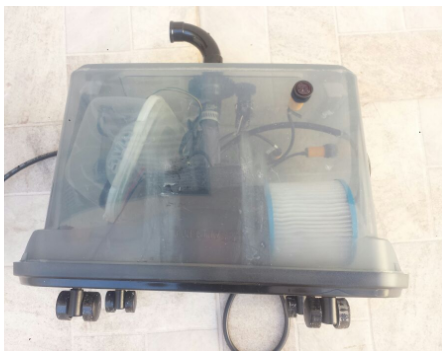
\includegraphics[width=0.5\textwidth]{figuras/cpr-02.png}
  \caption{Modelo CPR-02}
  \label{fig:cpr-02}
\end{figure}
\FloatBarrier

O CPR-02 de montagem foi aumentado do tamanho da carcaça definida no modelo anterior e adaptada de acordo com os tamanhos da caixa de vedação do circuito, bomba e filtros. Importante ressaltar que neste tópico foi mudado as rodas do robô para uma de plástico a fim de se evitar as possíveis corrosões já ocorridas no primeiro teste do sistema de locomoção. Juntamente com esse terceiro modelo, foi utilizado uma nova caixa para a colocação do circuito sendo esta adaptada somente a uma saída de fios e foi possível constatar que mais uma vez a vedação não foi suficiente, fazendo com que entrasse água na caixa. Para solucionar esse problema foi feita uma nova modelagem da caixa de processamento foi implementada no modelo CPR-03. O teste de integração esta etapa não se mostrou eficiente, visto que o robô não conseguiu alcançar o fundo da piscina devido ao materiais utilizados na parte interna do sistema de filtragem, além do fato da caixa de processamento, localizada dentro do robô, ter gerando uma espécie de bolha d’água interna a carcaça o que impediu de afundar.

O modelo CPR-03, foi construído de forma a garantir a completa inserção do robô na água. Para isso, alterou-se a estrutura do robô e adicionou furos para auxiliar na imersão do mesmo na água. O principal problema identificado no modelo anterior era a caixa de vedação que formava uma bolha d’água interna no modelo. O CPR-03 possui a caixa de vedação externa ao robô de forma a permanecer flutuando na superfície da água enquanto o robô realiza a limpeza. A idealização deste novo método focou em manter seguro o circuito de controle, bem como também todo o sistema envolvido e evitar o problema encontrado no  CPR-02.

\begin{figure}[h]
  \centering
  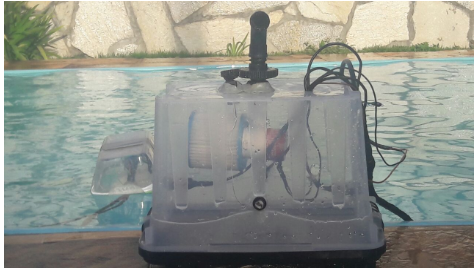
\includegraphics[width=0.6\textwidth]{figuras/cpr-03.png}
  \caption{Modelo CPR-03}
  \label{fig:cpr-03}
\end{figure}
\FloatBarrier

O modelo CPR-03 foi testado de forma integrada. A caixa de vedação e submersão do robô apresentou resultados positivos, além disso, testou-se o circuito fora da piscina e esse realizou o procedimento de forma adequada. Entretanto, o jato d’água não foi suficiente para permitir a locomoção esperada do robô. Com o teste, percebeu-se que o duto reduz a força do jato d’água de forma significativa.  Outra influência deve ser o peso da massa d’água não considerado para a movimentação do robô. Para o CPR-04, haverá algumas alterações de forma a permitir essa locomoção, entre elas a adição de uma bomba auxiliar, entretanto, até a entrega desse relatório, o CPR-04. A equipe espera resolver o problema da locomoção até a apresentação desse projeto.

\begin{figure}[h]
  \centering
  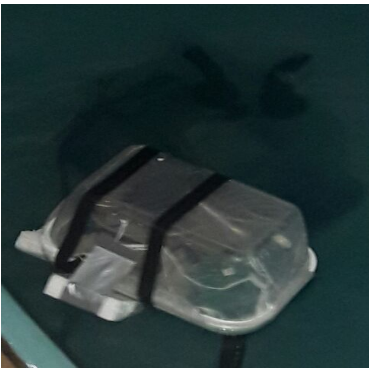
\includegraphics[width=0.4\textwidth]{figuras/cpr-04.png}
  \caption{CPR-03 em funcionamento}
  \label{fig:cpr-04}
\end{figure}
\FloatBarrier